\documentclass[10pt]{article}

\usepackage[margin=1in]{geometry}
\usepackage{amsmath,amssymb,amsthm,mathtools}
\usepackage{booktabs,array}
\usepackage{float}
\usepackage{graphicx}
\usepackage{microtype}
\usepackage[hidelinks]{hyperref}
\hypersetup{pdftitle={LSSO: Solved Contextual Operators for Bidirectional Sequence Modeling},
  pdfauthor={Zhaoyang Wang}}

\newtheorem{theorem}{Theorem}[section]
\newtheorem{proposition}[theorem]{Proposition}
\newtheorem{corollary}[theorem]{Corollary}
\newtheorem{definition}[theorem]{Definition}
\newtheorem{remark}[theorem]{Remark}

\newcommand{\R}{\mathbb{R}}
\newcommand{\I}{\mathbf{I}}
\newcommand{\T}{\mathsf{T}}
\newcommand{\norm}[1]{\left\lVert #1 \right\rVert}
\newcommand{\inner}[2]{\left\langle #1, #2 \right\rangle}
\newcommand{\rank}{\operatorname{rank}}
\newcommand{\sym}{\operatorname{sym}}
\newcommand{\diag}{\operatorname{Diag}}
\newcommand{\tril}{\operatorname{tril}}
\newcommand{\triu}{\operatorname{triu}}
\newcommand{\qf}{\operatorname{qf}}

\title{LSSO: Solved Contextual Operators for Bidirectional Sequence Modeling}
\author{Zhaoyang Wang\\\texttt{zhaoy@uir.edu.cn}}
\date{}

\begin{document}
\maketitle

\begin{abstract}
Bidirectional sequence models can use the entire context to construct a compact
state for global interaction.  Recent extensions of recurrent memory and
test-time training make this an increasingly useful alternative to dense
attention, but leave open how to jointly design the state, its induced mixing,
and its computational realization.  We introduce LSSO, a contextual operator
built around one compact direct solve per sample and head.  A full-context
cross-moment generates a strictly accretive system; its solved state is lifted
to tokens through a QR soft frame and a learned scalar complement.  The compact
core covers every real strict contraction, including nonsymmetric and nonnormal
maps, while the resulting token mixer has an exact gain computable in compact
space.  These guarantees concern the realized mixing operator, rather than the
end-to-end input-dependent network.  At fixed rank, arithmetic and activation
storage scale linearly with sequence length.  An algebraically equivalent CUDA
implementation evaluates the solve and its analytic backward without a dense
token map.  In a matched three-seed comparison on eight GenomicBenchmarks tasks,
LSSO obtains the highest mean accuracy on seven tasks and improves macro accuracy
from the strongest alternative's $75.57$ to $78.53$.  Additional long-sequence
results, trained-state diagnostics, and complete-mixer timings characterize the
scope and cost of this full-context design.
\end{abstract}

\begin{figure}[t]
\centering
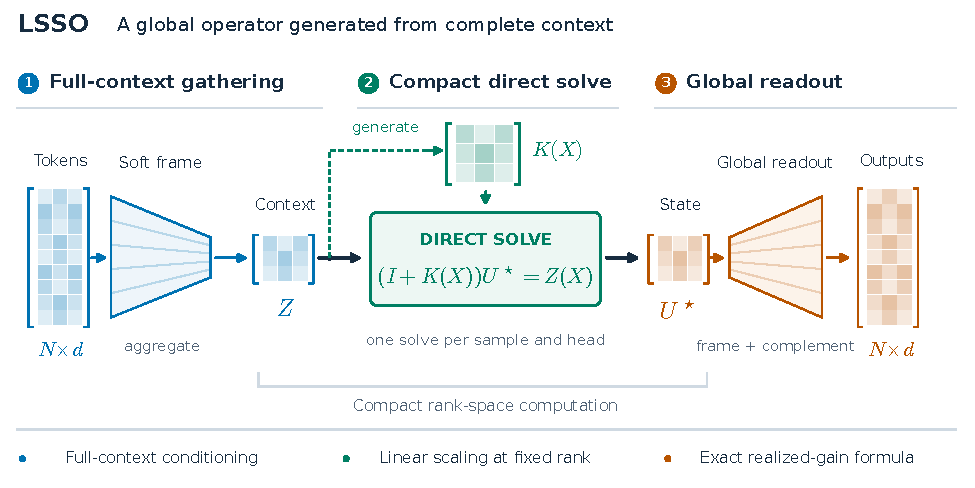
\includegraphics[width=\linewidth]{operator_overview.pdf}
\caption{\textbf{Graphical abstract: full context, compact solve, global mixing.}
All valid tokens jointly define a compact system.  One direct solve per sample
and head produces a shared state whose action reaches every output token.
At fixed rank, the construction scales linearly with sequence length and admits
an exact realized-gain formula.  This formula describes the mixer after freezing
its sample-conditioned quantities, not the end-to-end network Jacobian.
The dashed path generates the system from the context statistic; the solid
path evaluates it.  Global readout uses the shared frame, context statistic,
and scalar complement.  Tensor shapes are schematic; no experimental results
are depicted.}
\label{fig:overview}
\end{figure}

\section{Introduction}
\label{sec:introduction}

Image encoders and full-sequence classifiers receive all their tokens before
producing a prediction.  Each position can therefore draw on the entire sample,
which makes global interaction a natural building block.  Dense attention
provides this interaction through token pairs, but its quadratic arithmetic
becomes costly as the sequence grows.  Compact-state alternatives offer another
route: gather contextual information into a smaller representation and use it
to transform every token \cite{lee2019settransformer,ma2021luna,jaegle2021perceiver}.
The design of that representation determines both the global interaction and
its computational cost.

Recurrent linear attention, selective state-space models, and test-time
training (TTT) have developed powerful ways to construct such states from
context \cite{schlag2021fastweights,gu2024mamba,sun2025ttt}.
Their extension to bidirectional tasks is now an active architectural direction.
LION relates full, recurrent, and chunkwise forms of bidirectional linear
attention \cite{afzal2025lion}; ViT$^3$ studies full-batch inner updates for visual
TTT \cite{han2026vit3}; and ZipMap compresses an image collection into a shared
scene state for bidirectional reconstruction \cite{jin2026zipmap}.
These approaches establish several ways to exploit complete context.  In
particular, bidirectional information access and parallel execution are distinct
choices: a causal computation can be parallelized, and a bidirectional model
can retain directional scans.

When the entire context is available, a layer can construct its state jointly
from all tokens.  This raises a design question: \emph{what global transformation
should the state induce, and how should its expressivity, evaluation, and gain
be controlled?}  The optimization perspective of test-time regression provides
one framework for choosing a state \cite{wang2025testtimeregression}, and MesaNet
solves causal context regressions using conjugate gradients
\cite{vonoswald2026mesanet}.  However, a smaller inner loss need not imply better
task performance: recent analysis of KV-binding TTT motivates inspecting the
induced operator itself \cite{liu2026kvbinding}.  We consequently treat the
full-context operator as the design object, with its solve and geometry chosen
together.

LSSO constructs this operator from a compact strictly accretive system.  Each
head gathers the full sample into a cross-moment $Z=P^\T C$, generates a matrix
$K$ from $Z$, and obtains the contextual state by solving
$(\I+K)U^\star=Z$.  The state is read back through the same soft frame $P$ to
produce a global token transformation (Figure~\ref{fig:overview}).  Equivalently,
the compact action and its token-space lift are
\begin{align}
    M &= 2(\I+K)^{-1}-\I,
\label{eq:reflected-resolvent}\\
    T &= \eta\I+P(M-\eta\I)P^\T.
\label{eq:token-mixer-intro}
\end{align}
All valid tokens participate in generating this shared operator.  LSSO is a
native full-context construction, rather than an equivalence transformation of
an existing causal update rule.

The construction assigns a role to each structural choice.  Accretivity makes
the compact state uniquely solvable and controls the transposed solve used in
backpropagation.  Its reflected resolvent spans every strict contraction in
\emph{compact rank space}, so gain control still permits nonsymmetric mixing.
The soft frame lifts this action to tokens, while $\eta$ controls the complement
outside the frame.  Together they give an exact, sample-specific gain formula
using matrices no larger than $r\times r$.  Token--rank products and one small
direct solve realize the operator with linear sequence scaling at fixed rank;
the dense token matrix is never formed.

Our contributions are threefold:
\begin{enumerate}
    \item \textbf{A solved full-context operator.}  LSSO jointly constructs a
    compact state from all valid tokens and evaluates it by direct solution,
    without an inner learning rate, update schedule, or iterative stopping rule.
    \item \textbf{Expressive compact geometry with a computable global gain.}
    The compact chart covers the real strict matrix ball, and its structured
    token-space lift admits an exact realized-gain certificate.  A complementary
    monotonicity margin bounds the state and implicit adjoint.
    \item \textbf{Task evidence and efficient realization.}  Matched genomic
    experiments evaluate the complete mixer; LRA results and trained-state
    diagnostics examine further sequence settings.  An equivalent native CUDA
    implementation demonstrates the execution cost of the compact construction.
\end{enumerate}



\section{Related Work}
\label{sec:related-work}

\paragraph{Global compact-state mixing.}
Efficient Transformers replace the dense token map with projections,
landmarks, kernels, cosine reweighting, or inducing states
\cite{wang2020linformer,katharopoulos2020linear,
choromanski2021performer,qin2022cosformer,xiong2021nystrom}.  Set Transformer uses inducing
points for global set interaction \cite{lee2019settransformer}; Luna packs and
unpacks information through a fixed-length auxiliary sequence
\cite{ma2021luna}; and ABC interprets several such mechanisms as learned
bounded memory \cite{peng2022abc}.  Perceiver similarly mediates global
exchange through latent slots \cite{jaegle2021perceiver}.  LSSO advances this
compact-state line by building on XCiT's central insight that an
input-dependent cross-statistic can generate one compact global operator for
all tokens \cite{ali2021xcit}.  XCiT turns token-aggregated cross-covariance
into a shared channel mixer; LSSO carries the compact operator into token
space, where the cross-moment generates an accretive system.  Its equilibrium
is solved directly, and the resulting contraction is lifted through a learned
token frame without constructing a dense token matrix.

\paragraph{From causal memory to full-context operators.}
Fast-weight models and TTT construct a compact representation from a sequence
\cite{schlag2021fastweights,sun2025ttt}.  LION extends linear attention to
bidirectional tasks through equivalent full, recurrent, and chunkwise forms
\cite{afzal2025lion}.  ViT$^3$ studies full-batch visual inner updates
\cite{han2026vit3}, while ZipMap uses TTT to form a shared state from an image
collection \cite{jin2026zipmap}.  These are distinct ways to make complete
context available to the output.  LSSO contributes a different state
construction: a full-context statistic generates a compact system whose direct
solution defines the global mixing map.  The available experiments do not yet
compare LSSO against LION or visual TTT under a matched training protocol.

\begin{table}[t]
\centering
\small
\caption{Representative full-context constructions.  This comparison concerns
how the state is formed, not a matched performance ranking.}
\label{tab:full-context-designs}
\begin{tabular}{>{\raggedright\arraybackslash}p{0.18\linewidth}>{\raggedright\arraybackslash}p{0.31\linewidth}>{\raggedright\arraybackslash}p{0.40\linewidth}}
\toprule
Construction & Context representation & Evaluation route \\
\midrule
LION \cite{afzal2025lion} & Bidirectional linear-attention aggregates & Equivalent full, recurrent, or chunkwise forms \\
Visual full-batch TTT \cite{han2026vit3} & Updated inner-model parameters & Full-context inner update and query evaluation \\
LSSO & Generated compact system and solved state & Direct compact solve and soft-frame readout \\
\bottomrule
\end{tabular}
\end{table}

\paragraph{Context as a solved problem.}
Longhorn and test-time regression relate sequence processing to regression
objectives \cite{liu2024longhorn,wang2025testtimeregression}.  MesaNet optimizes
causal per-context regressions with a chunkwise conjugate-gradient formulation
\cite{vonoswald2026mesanet}.  Our bidirectional construction instead generates
one compact accretive problem per sample and head.  Its mathematical solution
is evaluated with a direct factorization, subject to floating-point error.
Analysis of KV-binding TTT further shows that inner optimization and task
performance need not track one another in the studied settings
\cite{liu2026kvbinding}.  This motivates our focus on the resulting operator;
we do not infer a task advantage merely from solving a system accurately.

\paragraph{Context-conditioned contractive geometry.}
S4 and selective state-space models obtain linear sequence scaling through
structured recurrence and input-dependent state evolution
\cite{gu2022s4,gu2024mamba,dao2024mamba2}.  Deep equilibrium models use
implicit differentiation at a root \cite{bai2019deep}; monotone operator
equilibrium networks additionally obtain well-posed states from monotone
structure \cite{winston2020mondeq}.  Direct Cayley parameterization gives a
complete trainable chart for static Lipschitz-bounded network weights
\cite{wang2023direct}.  LSSO makes this geometry contextual: every sample
generates a compact accretive operator, its exact solve produces the global
token mixer, and compact statistics recover the gain actually realized on
that sample.  Skew coordinates retain nonsymmetric and nonnormal
contractions.  This joins global noncausal conditioning with
accretive/resolvent geometry \cite{bauschke2017convex} and provides a directly
measurable operator guarantee in a setting where ordinary self-attention need
not be globally Lipschitz \cite{kim2021lipschitz}.

\paragraph{Hardware-efficient linear layers.}
FlashAttention demonstrated that avoiding materialized intermediates and
controlling memory traffic can matter as much as operation count
\cite{dao2022flashattention}; Mamba likewise couples its recurrence to a
hardware-aware parallel algorithm \cite{gu2024mamba}.  LSSO follows this
algorithm--implementation co-design principle.  Its native path lowers the
compact algebra to fused CUDA schedules for both the forward and analytic
backward.  Unlike exact softmax attention, whose pairwise arithmetic remains
quadratic even when FlashAttention avoids storing the score matrix, LSSO's
compact algebra is linear in sequence length at fixed rank.
Section~\ref{sec:cuda-implementation} reports its measured behavior, and
Appendix~\ref{app:cuda} gives the lowering and workspace accounting.

\section{LSSO}
\label{sec:method}

We describe one head and omit the batch index.  Let $X\in\R^{N\times D}$ be
the incoming token matrix, $d$ the head width, and $r$ the compact rank.  A
single input projection produces relation and content coordinates
\begin{equation}
    [A,C] = XW_{bc}+b_{bc},
    \qquad A\in\R^{N\times r},\quad C\in\R^{N\times d}.
\label{eq:input-projection}
\end{equation}
Heads are concatenated and passed through an ordinary output projection after
mixing.  The construction below is repeated independently for each head, with
one compact state shared by all valid tokens in that head.

\subsection{Full-context computation at a glance}
For normalized, position-transformed relation coordinates, LSSO builds a soft
frame $P$ and evaluates
\begin{equation}
 Z=P^\T C,\qquad U^\star=(\I_r+K(Z))^{-1}Z,\qquad
 Y=\eta C+P[2U^\star-(1+\eta)Z].
\label{eq:computation-overview}
\end{equation}
The first operation gathers the entire valid context; the second constructs a
shared solved state; the third returns its action to all tokens.  The following
subsections specify each operation.  Masking, $1/\sqrt n$ relation normalization,
and Rank-Rotary precede frame construction, as detailed in
Section~\ref{sec:mask-and-phase}; throughout, $n$ is the valid-token count.


\subsection{Gathering the full context into a compact statistic}
\label{sec:soft-frame}

The QR soft frame maps unconstrained relation coordinates to a strict column
contraction.  Form the reduced QR factorization
\begin{equation}
    \begin{bmatrix}P\\E\end{bmatrix}R_{\mathrm{qr}}
    =
    \begin{bmatrix}A\\\I_r\end{bmatrix},
    \qquad
    \begin{bmatrix}P\\E\end{bmatrix}^{\!\T}
    \begin{bmatrix}P\\E\end{bmatrix}=\I_r,
\label{eq:soft-frame}
\end{equation}
where $P\in\R^{N\times r}$ is the token-space frame.  A common positive
rescaling, which leaves the exact $Q$ factor unchanged, controls the numerical
range.
The identity augmentation means that the factorization is defined even when
$N<r$ or $A$ is rank deficient.

The frame compresses the content into one shared cross-moment,
\begin{equation}
    Z=P^\T C\in\R^{r\times d}.
\label{eq:cross-moment}
\end{equation}
$Z$ aggregates all valid positions symmetrically in one noncausal pass without
forming the token-level matrix in \eqref{eq:token-mixer-intro}.

\subsection{Generating and solving the contextual core}
\label{sec:accretive-core}

In the default \textsc{Dynamic} mode, $Z$ generates compact raw coordinates
\begin{equation}
    \Theta = \Theta_0 + \frac{ZW_{\mathrm{drive}}}{\sqrt{n}},
\label{eq:dynamic-coordinates}
\end{equation}
where $\Theta_0\in\R^{r\times r}$ and
$W_{\mathrm{drive}}\in\R^{d\times r}$ are learned per-head parameters.  The
\textsc{Static} ablation uses $\Theta=\Theta_0$, while \textsc{Zero} fixes the
compact contraction to zero.

For \textsc{Dynamic} and \textsc{Static}, define
\begin{align}
    L(\Theta) & = \tril(\Theta,-1)+
        \diag\!\left(\operatorname{softplus}
        \bigl(\operatorname{diag}(\Theta)+c_1\bigr)\right), \\
    \Omega(\Theta) & = \triu(\Theta,1)-\triu(\Theta,1)^\T, \\
    K(\Theta) & = L(\Theta)L(\Theta)^\T+\Omega(\Theta),
\label{eq:accretive-parameterization}
\end{align}
where $c_1=\operatorname{softplus}^{-1}(1)$.  Thus $L$ is lower triangular
with positive diagonal, while $\Omega$ is skew-symmetric.  The compact
equilibrium and the pre-output token coordinates are
\begin{align}
    U^\star &=(\I_r+K)^{-1}Z, \\
    Y &= \eta C+P\left[2U^\star-(1+\eta)Z\right],
    \qquad \eta=\tanh(\eta_{\mathrm{raw}})\in(-1,1).
\label{eq:equilibrium-readout}
\end{align}
The complement is learned independently for each head and is initialized to
$0.9$.  In \textsc{Zero}, $M=0$, which gives
\begin{equation}
    Y=\eta(C-PZ).
\label{eq:zero-core}
\end{equation}
At $\Theta=0$, $L=\I_r$, $\Omega=0$, $K=\I_r$, and the compact contraction is
$M=0$.  Both nonzero-core modes start at that point; \textsc{Dynamic} also
starts with $W_{\mathrm{drive}}=0$.

\subsection{Lifting the compact action to all tokens}

Define the reflected resolvent
\begin{equation}
    M = 2(\I_r+K)^{-1}-\I_r
      = (\I_r-K)(\I_r+K)^{-1}.
\label{eq:cayley}
\end{equation}
Substituting $Z=P^\T C$ into \eqref{eq:equilibrium-readout} gives the exact
token-mixing form
\begin{equation}
    Y=TC,\qquad
    T=\eta\I_N+P(M-\eta\I_r)P^\T.
\label{eq:token-mixer}
\end{equation}

\paragraph{Solved contextual inner state.}
LSSO obtains $U^\star$ by a direct $r\times r$ solve.
Appendix~\ref{sec:solved-inner-process} relates this solution to a globally
convergent contextual dynamics.

\subsection{Position, masking, and execution order}
\label{sec:mask-and-phase}

For a boolean validity mask $m\in\{0,1\}^N$, invalid rows of both $A$ and $C$
are set to zero before any compact statistic is formed.  Let
\begin{equation}
    n = \sum_{i=1}^N m_i.
\end{equation}
For a nonempty sequence, relation coordinates are normalized as
$A\leftarrow A/\sqrt{n}$.  An entirely masked sequence is assigned the zero
output by definition.  Masking before normalization makes the result invariant
to appended padding.

Rank-Rotary applies a block-diagonal planar rotation to
the $r$ relation coordinates before the soft frame.  For centered position
$p_i$ and frequencies $\{\omega_j\}_{j=1}^{r/2}$, each coordinate pair uses
the angle $p_i\omega_j$.  The transformation preserves each relation row's
Euclidean norm and obeys the relative-phase identity
\begin{equation}
    \mathcal R(p_i)^\T\mathcal R(p_j)=\mathcal R(p_j-p_i).
\label{eq:rank-rotary-relative}
\end{equation}
Rank-Rotary therefore supplies relative phase within relation rank space while
preserving each row norm.  Absolute or two-dimensional position embeddings
remain external to the mixer.  Full-context access does not remove positional
structure: these feature rotations are applied before aggregation and do not
impose a causal visibility mask.

\subsection{Linear sequence complexity}
\label{sec:linear-complexity}

For one head, frame formation costs $O(Nr^2)$, the two frame--content
contractions cost $O(Nrd)$, and construction and solution of the compact
problem cost $O(r^2d+r^3)$.  The forward arithmetic and activation/workspace
storage are therefore
\begin{align}
    \mathcal C_{\mathrm{LSSO}}
        &=O\!\left(Nr^2+Nrd+r^2d+r^3\right), \\
    \mathcal M_{\mathrm{LSSO}}
        &=O\!\left(N(r+d)+r^2+rd\right).
\label{eq:lsso-complexity}
\end{align}
The analytic backward reuses compact factors and performs the same classes of
token--rank contractions, so its arithmetic and saved-state dependence on $N$
is also linear.  Multiplying the head-local terms by the number of heads does
not change the sequence-length degree.

Unlike exact MHA, whose $O(N^2d)$ mixing cost persists under FlashAttention
\cite{dao2022flashattention}, LSSO has $O(Nr(r+d))$ token-dependent work and no
$N\times N$ intermediate.  Both retain $O(ND^2)$ feature projections.

\section{Geometry of the Full-Context Operator}
\label{sec:theory}

We analyze one realized head in exact arithmetic.  Complete proofs are given in
Appendix~\ref{app:proofs}, and mixed-precision execution is described in
Section~\ref{sec:cuda-implementation}.

\subsection{Is the contextual state well posed?}

\begin{theorem}[Stable solved state and implicit adjoint]
\label{thm:stable-solve}
Define the per-sample monotonicity margin
\begin{equation}
    \mu=1+\sigma_{\min}(L)^2>1,
    \qquad A_K=\I_r+K.
\label{eq:monotonicity-margin}
\end{equation}
Then $U^\star=A_K^{-1}Z$ exists uniquely, and
\begin{equation}
    \sigma_{\min}(A_K)\geq\mu,
    \quad
    \norm{U^\star}_F\leq\mu^{-1}\norm{Z}_F,
    \quad
    \norm{A_K^{-\T}G}_F\leq\mu^{-1}\norm{G}_F.
\label{eq:solve-adjoint-bound}
\end{equation}
For a second generated problem $A_K'=\I_r+K'$ with margin $\mu'$ and solution
$U^{\star'}=A_K'^{-1}Z'$, the finite contextual perturbation obeys
\begin{equation}
    \norm{U^\star-U^{\star'}}_F
    \leq \mu^{-1}\norm{Z-Z'}_F
       +(\mu\mu')^{-1}\norm{K-K'}_2\norm{Z'}_F.
\label{eq:finite-solve-sensitivity}
\end{equation}
Consequently, an infinitesimal perturbation obeys
\begin{equation}
    \norm{dU^\star}_F
    \leq \mu^{-1}\norm{dZ}_F
       +\mu^{-2}\norm{dK}_2\norm{Z}_F.
\label{eq:solve-sensitivity}
\end{equation}
\end{theorem}

The same computable margin controls the forward state, the transposed solve
used by implicit differentiation, and sensitivity to the generated compact
problem.  The realized-gain certificate below separately measures the
contraction margin, which also depends on the skew coordinates.

\subsection{What does gain control allow the operator to express?}

\paragraph{A frame that preserves the compact guarantee.}

\begin{theorem}[Soft-frame contract]
\label{thm:soft-frame}
Let $P$ be the upper block of the $Q$ factor in
\eqref{eq:soft-frame}.  If $\sigma_i(A)$ are the singular values of the
normalized relation matrix, then
\begin{equation}
    \sigma_i(P)=\frac{\sigma_i(A)}
    {\sqrt{1+\sigma_i(A)^2}}.
\label{eq:soft-frame-spectrum}
\end{equation}
Consequently,
\begin{equation}
    P^\T P \prec \I_r,
    \qquad
    \I_N-PP^\T \succ 0,
    \qquad
    1-\norm{P}_2^2=\frac{1}{1+\norm{A}_2^2}.
\label{eq:soft-frame-contract}
\end{equation}
Moreover, at the level of represented frames, the construction covers every
$P\in\R^{N\times r}$ satisfying $P^\T P\prec\I_r$.
\end{theorem}

\begin{proof}[Proof sketch]
The lower block of \eqref{eq:soft-frame} obeys
$ER_{\mathrm{qr}}=\I_r$.  Since the augmented matrix has full
column rank, $R_{\mathrm{qr}}$ and hence $E$ are nonsingular.  Orthogonality
of the full thin-$Q$ factor gives
\begin{equation}
    P^\T P+E^\T E=\I_r.
\end{equation}
Because $E^\T E\succ0$, the first claim follows.  Also
$R_{\mathrm{qr}}^\T R_{\mathrm{qr}}=\I_r+A^\T A$ and
$P=AR_{\mathrm{qr}}^{-1}$, which yields
\eqref{eq:soft-frame-spectrum} and the exact norm margin.  In particular,
$\norm{P}_2<1$, which implies $PP^\T\prec\I_N$ and proves the second claim.
\end{proof}

The identity augmentation supplies the strict complement $\I_N-PP^\T$, which
allows the compact contraction to extend to every token direction.  If $A_0$ denotes
the masked relation matrix before division by $\sqrt n$, the final term in
\eqref{eq:soft-frame-contract} becomes
$1/(1+\norm{A_0}_2^2/n)$.  Thus bounded per-token relation energy prevents the
frame margin from deteriorating merely because the sequence is longer.

\begin{proposition}[Length-normalized contextual drive]
\label{prop:length-normalized-drive}
For the dynamic core,
\begin{equation}
    \norm{Z}_F\leq\norm{P}_2\norm{C}_F,
    \qquad
    \norm{\Theta-\Theta_0}_F
    \leq \frac{\norm{C}_F}{\sqrt n}\norm{W_{\mathrm{drive}}}_2.
\label{eq:length-normalized-drive}
\end{equation}
The first inequality is strict relative to $\norm{C}_F$ whenever $C\neq0$.
Accordingly, if $\norm{C}_F^2/n\leq c^2$, the magnitude of the contextual
drive is at most $c\norm{W_{\mathrm{drive}}}_2$, independently of sequence
length.
\end{proposition}

\paragraph{A complete compact contraction chart.}

\begin{definition}[Strict accretivity]
\label{def:accretive}
A real square matrix $K$ is strictly accretive when
\begin{equation}
    \sym(K) \coloneqq \frac{K+K^\T}{2}\succ0.
\end{equation}
\end{definition}

The Cayley connection between accretive coordinates and contractions is
classical in monotone operator theory \cite{bauschke2017convex}, and direct
Cayley charts have parameterized static Lipschitz-bounded network weights
\cite{wang2023direct}.  The result below gives the complete strict form needed
by LSSO.  Its role here is contextual: $K$ is generated from the current
sample's cross-moment, and the resulting contraction is lifted through that
sample's token frame.

\begin{theorem}[Accretive Cayley parameterization]
\label{thm:accretive-cayley}
The map in \eqref{eq:accretive-parameterization} ranges over all real
strictly accretive $r\times r$ matrices.  For every such $K$, the reflected
resolvent $M$ in \eqref{eq:cayley} is a strict spectral-norm contraction and
obeys
\begin{equation}
    \I_r-M^\T M
    =4(\I_r+K)^{-\T}L L^\T(\I_r+K)^{-1}\succ0.
\label{eq:cayley-defect}
\end{equation}
Conversely, the map $K\mapsto M$ is a bijection from real strictly accretive
matrices to the open real matrix ball $\{M:\norm{M}_2<1\}$, with inverse
\begin{equation}
    K=(\I_r-M)(\I_r+M)^{-1}.
\label{eq:inverse-cayley}
\end{equation}
\end{theorem}

\begin{proof}[Proof sketch]
The construction has
$\sym(K)=LL^\T\succ0$, because $L$ has positive diagonal.  Conversely, for
any strictly accretive $K$, the Cholesky factor of $\sym(K)$ and the skew
remainder $K-\sym(K)$ recover $L$ and $\Omega$, proving completeness.

Let $Q=\I_r+K$.  Strict accretivity implies that $Q$ is nonsingular.  Using
$M=(\I_r-K)Q^{-1}$ gives
\begin{align}
    \I_r-M^\T M
    &=Q^{-\T}\left[Q^\T Q-(\I_r-K)^\T(\I_r-K)\right]Q^{-1}\\
    &=4Q^{-\T}\sym(K)Q^{-1},
\end{align}
which is \eqref{eq:cayley-defect}.  It is positive definite, so
$\norm{M}_2<1$.
The inverse formula maps every strict contraction back to a strictly
accretive matrix.
\end{proof}

Because $\Omega$ is unrestricted, $K$ and $M$ may be nonsymmetric and
nonnormal.  The chart retains every strict contraction in rank space, and at
token level,
$T-T^\T=P(M-M^\T)P^\T$, so this nonsymmetric structure survives the lift.

\subsection{Can the realized global gain be computed exactly?}

The soft frame identifies the token subspace where contextual mixing acts.
Figure~\ref{fig:geometry} separates this compact action from the scalar
complement.  Because $P$ is generally not orthonormal, the restricted token
block $B$ below differs from the compact Cayley core $M$.

\begin{figure}[t]
\centering
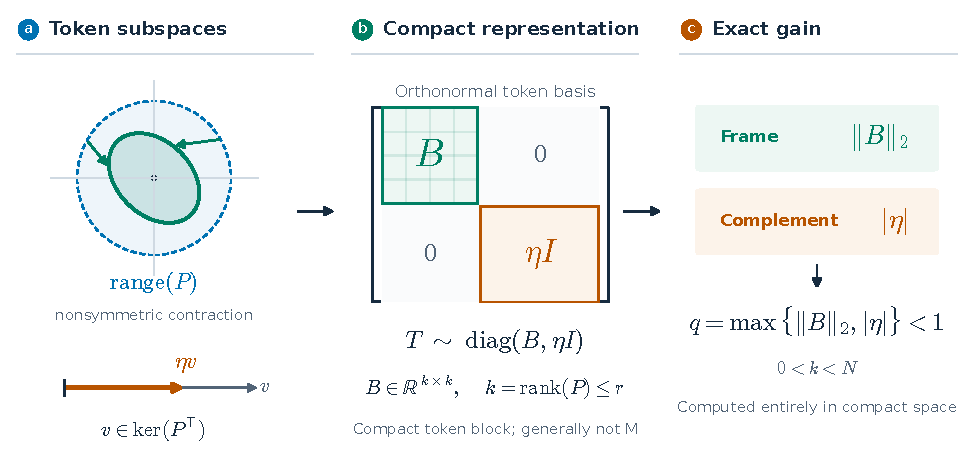
\includegraphics[width=\linewidth]{operator_geometry.pdf}
\caption{\textbf{From token subspaces to an exact gain.}
(a) An illustrative nonsymmetric contraction in the frame subspace and scalar
multiplication on its orthogonal complement; the scalar sketch uses positive
$\eta$.  (b) In an orthonormal token basis, the realized mixer separates into
$B$ and $\eta I$.  (c) For $0<k<N$, its norm is the larger of the two block norms.
Theorem~\ref{thm:token-contraction} covers either sign of $\eta$ and the empty
and full-rank cases.  The ellipse and matrix glyphs are schematic, not trained
operator measurements.}
\label{fig:geometry}
\end{figure}


\begin{theorem}[Exact realized-gain certificate]
\label{thm:token-contraction}
Fix a sample and head, and let $P$, $M$, and $\eta$ be constructed as above.
Write the positive eigenspace of $P^\T P$ as
\begin{equation}
    P^\T P=V_kS^2V_k^\T,
    \qquad k=\rank(P),
\end{equation}
where $S\in\R^{k\times k}$ is positive diagonal, and define
\begin{equation}
    B=\eta\I_k+SV_k^\T(M-\eta\I_r)V_kS.
\label{eq:compact-certificate-block}
\end{equation}
Then the singular values of $T$ are exactly those of $B$, together with
$N-k$ copies of $|\eta|$.  Equivalently,
\begin{equation}
 q(X)\coloneqq\norm{T}_2=
 \begin{cases}
   |\eta|, & k=0,\\
   \sigma_{\max}(B), & k=N,\\
   \max\{\sigma_{\max}(B),|\eta|\}, & 0<k<N,
 \end{cases}
 \qquad q(X)<1.
\label{eq:exact-token-gain}
\end{equation}
Moreover, $\rank(T-\eta\I_N)\leq r$ and
$Tv=\eta v$ for every $v\in\ker(P^\T)$.
\end{theorem}

\begin{proof}[Proof sketch]
Let $Q=PV_kS^{-1}$.  Then $Q^\T Q=\I_k$, and substitution gives
$T=QBQ^\T+\eta(\I_N-QQ^\T)$, so an orthogonal basis containing $Q$ yields the
stated singular spectrum.  With $\Delta=(\I_N-PP^\T)^{1/2}$ and
$F=[P\;\Delta]$,
\begin{equation}
    T=F\diag(M,\eta\I_N)F^\T,
\label{eq:defect-completion}
\end{equation}
and $FF^\T=\I_N$; hence $\norm{T}_2<1$.  Finally,
$T-\eta\I_N=P(M-\eta\I_r)P^\T$, which gives both the rank bound and
$Tv=\eta v$ on $\ker(P^\T)$.
\end{proof}

The exact certificate requires only an
$r\times r$ Gram eigendecomposition and a singular-value calculation of size
at most $r\times r$; no $N\times N$ kernel is needed.  Because the forward uses the
input-dependent $T(X)$ itself, Equation~\eqref{eq:exact-token-gain} gives the
pointwise energy statement
\begin{equation}
    \norm{T(X)C(X)}_F\leq q(X)\norm{C(X)}_F<\norm{C(X)}_F
\label{eq:pointwise-energy}
\end{equation}
whenever $C(X)\neq0$.  The guarantee is pointwise in the input-conditioned
operator.  It does not bound the Jacobian of $X\mapsto T(X)C(X)$,
which also contains $(dT)C$.  Along any fixed realized sequence of mixer maps, the gains compose:
$\norm{T_L\cdots T_1}_2\leq\prod_{\ell=1}^L q_\ell$.

\begin{remark}[Why the scalar complement is part of the model]
\label{rem:complement}
Without the complement, a conventional form $\I_N+PAP^\T$ fixes the entire
$\ker(P^\T)$ subspace to gain one.  Equation~\eqref{eq:defect-completion}
instead assigns that unmodeled subspace the learned per-head scalar $\eta$,
while retaining the same rank-$r$ correction and the strict contraction
certificate.  Thus $T$ is a rank-$r$ correction to an isotropic complement.
\end{remark}

Appendix~\ref{app:proofs} proves padding isolation and noncausal permutation
equivariance.

\section{Task Evidence and Realized Operators}
\label{sec:sequence-experiments}

We evaluate LSSO as a drop-in replacement for attention in otherwise ordinary
bidirectional encoders.  All reported LSSO runs use the default
\textsc{Dynamic} core, Rank-Rotary, rank $32$, FP16
automatic mixed precision, and the CUDA implementation.  Checkpoints are
selected only by validation accuracy, with validation loss breaking an exact
tie; the held-out test split is evaluated once after selection.  Reported
uncertainties are sample standard deviations over seeds $0$, $1$, and $2$.
Across the evaluated task configurations, LSSO requires only
$1.3\%$--$32.0\%$ of exact MHA's sequence-dependent mixer-core MACs
(Appendix~\ref{app:mixer-macs}).

\subsection{Matched genomic mixer comparison}

GenomicBenchmarks collects binary DNA sequence-classification tasks with
official train and test partitions \cite{gresova2023genomicbenchmarks}.  We
derive a deterministic stratified validation set only from each training
partition.  All mixers use the same $D=128$, four-layer, four-head encoder,
learned absolute position embeddings, MLP ratio $4$, mean readout, optimizer,
data order, and $40$-epoch budget; only the token mixer changes.  Alongside MHA,
we test bidirectional ELU${}+1$ Linear Transformer
\cite{katharopoulos2020linear}, FAVOR$+$ Performer with fixed orthogonal
random features \cite{choromanski2021performer}, and the official bidirectional
ReLU/cosine cosFormer formulation \cite{qin2022cosformer}.  Numerically
sensitive attention cores run in FP32 under automatic mixed precision.  The
effective batch is $128$, using two-step accumulation for Mouse Enhancers
Ensembl.  The three linear baselines match MHA's parameter count; LSSO is
$4.1\%$ smaller on the 200-position tasks.

\begin{table}[H]
\centering
\footnotesize
\setlength{\tabcolsep}{3.2pt}
\caption{GenomicBenchmarks held-out test accuracy (\%), mean $\pm$ sample
standard deviation over three seeds under the matched encoder and training
protocol.  Bold marks the highest mean in each row.}
\label{tab:genomic-results}
\begin{tabular}{lrrrrr}
\toprule
Task & MHA & Linear & Performer & cosFormer & LSSO \\
\midrule
Coding vs. intergenomic  & $80.34\pm1.99$ & $78.11\pm0.10$ & $78.17\pm0.01$ & $79.12\pm0.05$ & $\boldsymbol{83.23\pm2.46}$ \\
Human or worm            & $65.87\pm0.35$ & $65.68\pm0.22$ & $65.76\pm0.08$ & $66.07\pm0.20$ & $\boldsymbol{81.57\pm1.18}$ \\
Mouse enhancers Ensembl  & $71.07\pm1.65$ & $\boldsymbol{71.63\pm0.48}$ & $71.35\pm0.48$ & $71.35\pm0.48$ & $70.25\pm0.83$ \\
Human enhancers Cohn     & $66.83\pm0.17$ & $66.89\pm0.07$ & $67.16\pm0.08$ & $67.06\pm0.23$ & $\boldsymbol{67.24\pm0.26}$ \\
Human enhancers Ensembl  & $76.37\pm0.20$ & $75.16\pm0.57$ & $74.32\pm0.23$ & $77.34\pm1.53$ & $\boldsymbol{78.91\pm0.05}$ \\
Human regulatory         & $92.14\pm0.05$ & $91.79\pm0.15$ & $90.10\pm0.34$ & $92.65\pm0.14$ & $\boldsymbol{93.10\pm0.02}$ \\
Human non-TATA promoters & $84.71\pm0.15$ & $80.44\pm1.84$ & $82.51\pm1.07$ & $84.42\pm0.48$ & $\boldsymbol{85.41\pm0.17}$ \\
Human OCR Ensembl        & $65.61\pm0.54$ & $65.12\pm0.26$ & $65.36\pm0.27$ & $66.56\pm0.07$ & $\boldsymbol{68.55\pm0.31}$ \\
\midrule
Unweighted task macro    & $75.37$ & $74.35$ & $74.34$ & $75.57$ & $\mathbf{78.53}$ \\
\bottomrule
\end{tabular}
\end{table}

Table~\ref{tab:genomic-results} shows that LSSO has the highest mean on
seven of eight tasks; this is not a claim of statistical significance on each task.  Its $78.53$ macro average exceeds cosFormer, the strongest alternative
at $75.57$, by $2.96$ points and MHA's $75.37$ by $3.16$ points.  The three
linear-attention controls indicate that neither removing softmax nor obtaining
linear sequence scaling alone reproduces LSSO's gain.  The macro result first
averages seeds within each task and then gives all tasks equal weight.  The
largest gain occurs on Human or Worm; Mouse Enhancers Ensembl is the sole
exception, where Linear Transformer is highest.

\subsection{Scope of mechanism attribution}
The matched comparison tests the complete LSSO layer.  It does not isolate the
benefits of the dynamic drive, skew coordinates, rank, or Rank-Rotary.
In particular, \textsc{Static} removes the dynamic drive to $K$ while leaving
$P$ input-dependent; it is not a fully input-independent mixer.  Matched
\textsc{Dynamic}/\textsc{Static}/\textsc{Zero} training and core-activity
measurements are needed to attribute a task advantage to the generated core.
No such ablation results are included here.

\subsection{Certificates in trained models}
\label{sec:certificate-evidence}

We next measure how much certified margin trained models retain.  Across three
six-layer LRA Text checkpoints and matched held-out token-stream probes from
$1$K to $8$K, all $9{,}216$ head-level observations are finite and satisfy
their certified conditions (Table~\ref{tab:certificate-audit}).  The worst
realized gain is $0.9087$, leaving at least $0.0913$ contraction slack, and the
minimum monotonicity margin is $1.1667$.  Solved states use at most $93.3\%$ of
their certified bound, while deterministic adjoint probes use at most $88.1\%$.
Appendix~\ref{app:certificate-protocol} reports the per-layer distributions
and stress-test protocol.

\begin{table}[H]
\centering
\small
\setlength{\tabcolsep}{7pt}
\caption{Worst observation in the trained-model certificate audit.  Bound
usage is the measured ratio normalized by its certified upper bound $1/\mu$.}
\label{tab:certificate-audit}
\begin{tabular}{lcc}
\toprule
Quantity & Certified condition & Worst observed \\
\midrule
Realized gain & $q(X)<1$ & $\max q=0.9087$ \\
Contraction slack & $1-q(X)>0$ & $\min(1-q)=0.0913$ \\
Monotonicity margin & $\mu>1$ & $\min\mu=1.1667$ \\
Solved-state bound usage & $\mu\norm{U^\star}_F/\norm{Z}_F\leq1$ & $0.9329$ \\
Adjoint-probe bound usage & $\mu\norm{A_K^{-\T}G}_F/\norm{G}_F\leq1$ & $0.8814$ \\
\bottomrule
\end{tabular}
\end{table}


The gain in these probes is dominated by the scalar complement $|\eta|$
(Appendix~\ref{app:certificate-protocol}).  The audit therefore establishes
realized operator margins, not the task contribution of the dynamic core.
The $8$K probes are operator stress tests on assembled token streams, not an
$8$K classification or length-generalization result.

\subsection{Long Range Arena context}

Long Range Arena (LRA) tests structured reasoning and long-context
classification \cite{tay2021lra}.  Following established reporting practice
\cite{gu2022s4}, Table~\ref{tab:lra-results} quotes results from the original
benchmark and subsequent work and groups models by their primary mixing
mechanism.  General-purpose global mixers and efficient-attention
approximations form the first block; structured recurrence and state-space
models form the second.  This distinction matters because explicit locality
and positional structure materially affect LRA performance
\cite{mirallesgonzalez2025locality}.

We evaluate LSSO on four LRA tasks using six-layer encoders, with $D=128$ for
ListOps and Retrieval and $D=256$ for Text and Pathfinder-32.  ListOps, Text,
and Retrieval use learned one-dimensional absolute position embeddings with
mean pooling; Pathfinder-32 uses factorized row/column embeddings and
mean--maximum pooling.  Their maximum sequence lengths are $2048$, $4096$,
$4000$, and $1024$, respectively.

\begin{table}[H]
\centering
\footnotesize
\setlength{\tabcolsep}{2.5pt}
\caption{LRA test accuracy (\%) quoted from the cited sources under their
reported protocols.  The four-task average is unweighted over the displayed
tasks.  For LSSO, task scores and the per-seed four-task average are reported as
mean $\pm$ sample standard deviation across three seeds.  Bold marks the
highest reported mean within each mechanism block.}
\label{tab:lra-results}
\begin{tabular}{lrrrrr}
\toprule
Model and source & ListOps & Text & Retrieval & Pathfinder & 4-task Avg. \\
\midrule
\multicolumn{6}{l}{\emph{General-purpose global mixers and efficient-attention approximations}} \\
Transformer \cite{tay2021lra} & $36.37$ & $64.27$ & $57.46$ & $71.40$ & $57.38$ \\
Linear Transformer \cite{tay2021lra} & $16.13$ & $\mathbf{65.90}$ & $53.09$ & $75.30$ & $52.61$ \\
Performer \cite{tay2021lra} & $18.01$ & $65.40$ & $53.82$ & $77.05$ & $53.57$ \\
Linformer \cite{tay2021lra} & $35.70$ & $53.94$ & $52.27$ & $76.34$ & $54.56$ \\
Reformer \cite{tay2021lra} & $37.27$ & $56.10$ & $53.40$ & $68.50$ & $53.82$ \\
Luna-256 \cite{ma2021luna}
    & $\mathbf{37.98}$ & $65.78$ & $79.56$ & $78.55$ & $65.47$ \\
FNet \cite{leethorp2022fnet} & $35.33$ & $65.11$ & $59.61$ & $77.80$ & $59.46$ \\
Nystr\"omformer \cite{xiong2021nystrom}
    & $37.15$ & $65.52$ & $79.56$ & $70.94$ & $63.29$ \\
\textbf{LSSO}, three seeds
    & $37.60\pm0.65$ & $65.19\pm0.46$ & $\boldsymbol{82.88\pm0.08}$
    & $\boldsymbol{78.79\pm0.34}$ & $\boldsymbol{66.11\pm0.24}$ \\
\midrule
\multicolumn{6}{l}{\emph{Models centered on structured recurrence or state-space dynamics}} \\
S4, original \cite{gu2022s4}  & $58.35$ & $76.02$ & $87.09$ & $86.05$ & $76.88$ \\
S4-LegS, updated \cite{gu2022hippo}
    & $59.60\pm0.07$ & $86.82\pm0.13$ & $90.90\pm0.15$ & $94.20\pm0.25$ & $82.88$ \\
Mega \cite{ma2023mega} & $\mathbf{63.14}$ & $\mathbf{90.43}$
    & $\mathbf{91.25}$ & $\mathbf{96.01}$ & $\mathbf{85.21}$ \\
\bottomrule
\end{tabular}
\end{table}

Within the global-mixer block, LSSO gives the highest Retrieval, Pathfinder,
and four-task average; it is within $0.38$ points of the highest ListOps result
and $0.71$ points of the highest Text result.  The same mixer spans symbolic,
byte-level, paired-retrieval, and two-dimensional path tasks.

\section{Execution Cost of the Solved Operator}
\label{sec:cuda-implementation}

The default \textsc{Dynamic} core with Rank-Rotary has a native,
algebraically equivalent CUDA path for inference and first-order training.  It
avoids both the $N\times N$ token matrix and the compact Cayley matrix; compact
factorization and tiled solves evaluate the equilibrium directly, while the
analytic backward reuses saved factors.  Mixed-precision outputs and gradients
are validated against the FP64 reference.  Appendix~\ref{app:cuda} gives the
execution schedule, workspace, VJP, numerical envelope, and build coverage.

The following measurements use the historical contract-6 implementation;
they have not been rerun under the current contract-8 mixed-precision backend.
Table~\ref{tab:cuda-wall-clock} measures the complete mixer boundary, including
input and output projections.  At $N=4096$, native LSSO reaches $1.79\times$
the Flash-SDPA MHA forward throughput and $2.30\times$ its training throughput.
Across $N=1024$--$4096$, forward--backward latency grows by $3.88\times$ for
LSSO and $7.92\times$ for MHA.  These finite-shape timings illustrate
the scaling trend; they are not an asymptotic fit or an end-to-end model benchmark.

\begin{table}[H]
\centering
\footnotesize
\setlength{\tabcolsep}{4pt}
\caption{Synchronized milliseconds per batch on an RTX 5070 Ti (lower is
better), with $B=64,D=256,H=8$, FP16 AMP, and $r=32$ for LSSO
(historical contract 6).  Ratios above
one favor native LSSO; forward--backward includes loss and gradient reset.
Bold marks the lowest latency in each row.}
\label{tab:cuda-wall-clock}
\begin{tabular}{lrrrrr}
\toprule
$N$ & PyTorch ref. & Native & MHA & Ref./native & MHA/native \\
\midrule
\multicolumn{6}{l}{\emph{Inference forward}} \\
1024 & 110.216 & 2.539  & $\mathbf{2.131}$  & $43.41\times$ & $0.84\times$ \\
2048 & 133.940 & $\mathbf{5.577}$  & 5.888  & $24.02\times$ & $1.06\times$ \\
4096 & 169.549 & $\mathbf{10.135}$ & 18.173 & $16.73\times$ & $1.79\times$ \\
\midrule
\multicolumn{6}{l}{\emph{Forward--backward with gradient reset}} \\
1024 & 118.858 & $\mathbf{7.512}$  & 8.487  & $15.82\times$ & $1.13\times$ \\
2048 & 153.955 & $\mathbf{15.260}$ & 22.940 & $10.09\times$ & $1.50\times$ \\
4096 & 211.268 & $\mathbf{29.160}$ & 67.195 & $7.25\times$  & $2.30\times$ \\
\bottomrule
\end{tabular}
\end{table}

\section{Visual Representation and Dense Prediction}
\label{sec:vision}
% Intentionally empty: no visual results are claimed in this draft.
\subsection{ImageNet classification}
\subsection{COCO detection and instance segmentation}
\subsection{ADE20K semantic segmentation}

\section{Limitations}
\label{sec:limitations}

LSSO is designed for bidirectional tasks: its compact statistic uses the full
valid sequence.  It has no causal masking or autoregressive decoding contract.
The token-space family is a rank-$r$ correction to a scalar complement, even
though the compact chart covers every real strict contraction.  Its realized
gain certificate does not bound the end-to-end Jacobian, which also includes
derivatives of the input-conditioned operator, feature projections, and the
surrounding network.

The task evidence evaluates the complete layer on genomic classification and
four LRA tasks.  Mechanism attribution, matched comparisons with recent
bidirectional linear attention and TTT, and visual transfer remain open.
The native packages support $r\in\{16,32,48,64\}$, but the reported task runs
use $r=32$.  Timings are hardware- and shape-specific and use the historical
implementation contract; broader hardware, rank, and current-backend
measurements are needed to extend those empirical conclusions.

\section{Conclusion}

Complete context permits a sequence layer to construct its mixing state jointly
from all tokens.  LSSO realizes this choice through a sample-generated compact
system and one direct solve.  The accretive core, soft frame, and scalar
complement jointly specify an expressive compact action, a structured global
lift, and an exactly computable realized gain.  The resulting algebra supports
linear sequence scaling at fixed rank and an equivalent native backward.
Matched genomic results establish task value for the complete layer, while
long-sequence diagnostics and timings characterize its realized behavior.
This construction makes the full-context operator, its geometry, and its
execution part of the same design.

\appendix

\section{Complete Theoretical Details}
\label{app:proofs}

\subsection{Soft-frame spectrum and coverage}

Let $A=U\Sigma V^\T$ be an SVD of the normalized relation matrix.  From the
positive-diagonal QR factorization in \eqref{eq:soft-frame},
\begin{equation}
    R_{\mathrm{qr}}^\T R_{\mathrm{qr}}=\I_r+A^\T A,
    \qquad P=AR_{\mathrm{qr}}^{-1}.
\end{equation}
Hence
\begin{equation}
    PP^\T=A(\I_r+A^\T A)^{-1}A^\T
       =U\diag\!\left(
       \frac{\sigma_i(A)^2}{1+\sigma_i(A)^2}\right)U^\T.
\end{equation}
This proves \eqref{eq:soft-frame-spectrum}, including rank-deficient $A$ and
$N<r$.  The Cholesky/QR coordinates may differ from the symmetric-square-root
form $A(\I_r+A^\T A)^{-1/2}$ by a right orthogonal factor, while their singular
spectra and left Gram matrices agree.

Take any $P\in\R^{N\times r}$ with $P^\T P\prec\I_r$ and write
$S=\I_r-P^\T P\succ0$.  Let $C$ be the upper-triangular Cholesky factor of
$S$, so $S=C^\T C$, and set $R_{\mathrm{qr}}=C^{-1}$ and
$A=PR_{\mathrm{qr}}$.  Then
\begin{equation}
    \begin{bmatrix}A\\\I_r\end{bmatrix}
    =
    \begin{bmatrix}P\\R_{\mathrm{qr}}^{-1}\end{bmatrix}R_{\mathrm{qr}}.
\end{equation}
The left factor has orthonormal columns because
$R_{\mathrm{qr}}^{-\T}R_{\mathrm{qr}}^{-1}=S$.  It is therefore the unique
positive-diagonal reduced QR factorization and produces the desired upper
block $P$.

\subsection{Converse Cayley map and solve bound}

For any $M$ with $\norm{M}_2<1$, the matrix $\I_r+M$ is nonsingular.  Define
$K=(\I_r-M)(\I_r+M)^{-1}$.  Direct substitution gives
\begin{equation}
    K+K^\T
    =2(\I_r+M)^{-\T}(\I_r-M^\T M)(\I_r+M)^{-1}\succ0.
\end{equation}
Thus $K$ is strictly accretive, and the forward and inverse
fractional-linear expressions are algebraic inverses wherever defined.

Let $\mu$ be defined in \eqref{eq:monotonicity-margin}.  For a nonzero $v$,
the skew part of $K$ contributes zero to the quadratic form, so
\begin{equation}
    \inner{(\I_r+K)v}{v}
    =\norm{v}_2^2+\norm{L^\T v}_2^2\geq\mu\norm{v}_2^2.
\end{equation}
Cauchy--Schwarz therefore gives
$\norm{(\I_r+K)v}_2\geq\mu\norm{v}_2$, proving
$\sigma_{\min}(\I_r+K)\geq\mu$ and
$\norm{(\I_r+K)^{-1}}_2\leq\mu^{-1}$.

\subsection{The direct solve resolves a convergent contextual process}
\label{sec:solved-inner-process}

Let $A_K=\I_r+K$.  The following result relates the direct solve to a
continuous contextual process.

\begin{theorem}[Solved contextual inner process]
\label{thm:inner-process}
For fixed contextual quantities $K$ and $Z$, consider the continuous dynamics
\begin{equation}
    \dot U(t)=Z-A_KU(t).
\label{eq:contextual-flow}
\end{equation}
From every initial state $U(0)$, the dynamics converge to
$U^\star=A_K^{-1}Z$ and obey
\begin{equation}
    \norm{U(t)-U^\star}_F
    \leq e^{-\mu t}\norm{U(0)-U^\star}_F.
\label{eq:flow-rate}
\end{equation}
The rate lower bound is independent of the skew-symmetric part of $K$.

\end{theorem}

\begin{proof}[Proof sketch]
Write $E(t)=U(t)-U^\star$.  Since $A_KU^\star=Z$,
$\dot E=-A_KE$.  The skew part vanishes in the Frobenius inner product, so
\begin{equation}
    \frac{d}{dt}\frac12\norm{E}_F^2
    =-\inner{E}{A_KE}_F
    =-\inner{E}{\sym(A_K)E}_F
    \leq-\mu\norm{E}_F^2,
\end{equation}
because $\sym(A_K)=\I_r+LL^\T\succeq\mu\I_r$.  Gronwall's inequality gives
\eqref{eq:flow-rate}.
\end{proof}

Appendix~\ref{app:proofs} also identifies the direct solution as the
infinite-step limit of stable gradient descent on the residual objective.  The
production backward differentiates this solved state rather than a finite
unroll.

\subsection{Residual optimization, implicit derivative, and sensitivity}

The solved state also uniquely minimizes
\begin{equation}
    J(U)=\frac12\norm{A_KU-Z}_F^2,
    \qquad A_K=\I_r+K,
\label{eq:residual-objective}
\end{equation}
whose Hessian is $A_K^\T A_K\succ0$.  Gradient descent with
$0<\alpha<2/\sigma_{\max}(A_K)^2$ obeys
\begin{equation}
    \norm{U_j-U^\star}_F
    \leq\rho^j\norm{U_0-U^\star}_F,
    \qquad
    \rho=\max_i|1-\alpha\sigma_i(A_K)^2|<1.
\end{equation}
Hence the direct solve is both the infinite-time limit in
Theorem~\ref{thm:inner-process} and the infinite-step limit of every such
residual-gradient run.

Differentiating $A_KU^\star=Z$ gives
\begin{equation}
    dU^\star=A_K^{-1}(dZ-dA_K\,U^\star).
\label{eq:equilibrium-differential}
\end{equation}
If $G=\partial\mathcal L/\partial U^\star$ and $V=A_K^{-\T}G$, trace
cyclicity yields the exact implicit VJP
\begin{equation}
    \frac{\partial\mathcal L}{\partial Z}=V,
    \qquad
    \frac{\partial\mathcal L}{\partial A_K}=-VU^{\star\T}.
\label{eq:implicit-vjp}
\end{equation}
For two generated problems, the resolvent identity gives
\begin{align}
    U^\star-U^{\star'}
    &=A_K^{-1}(Z-Z')
      +A_K^{-1}(K'-K)A_K'^{-1}Z',
\end{align}
which proves \eqref{eq:finite-solve-sensitivity}.  Taking its differential
gives \eqref{eq:equilibrium-differential} and the stated local bound.
The solve and adjoint bounds above further give
\begin{equation}
    \norm{U^\star}_F\leq\mu^{-1}\norm{Z}_F,
    \qquad
    \norm{V}_F\leq\mu^{-1}\norm{G}_F,
    \qquad
    \norm{dU^\star}_F
    \leq\mu^{-1}\norm{dZ}_F
      +\mu^{-2}\norm{dK}_2\norm{Z}_F.
\end{equation}

The margin $\mu$ certifies the solve and flow rate, while the realized-gain
certificate separately captures the effect of skew coordinates.  For example,
with $L=\I_2$ and
$\Omega=a\left[\begin{smallmatrix}0&-1\\1&0\end{smallmatrix}\right]$,
$\mu=2$ for every $a$, while the associated $\norm{M}_2$ approaches one as
$|a|\to\infty$.  This is why the realized token gain is computed separately
by \eqref{eq:exact-token-gain}.

\subsection{Exact compact token spectrum}

With the notation of Theorem~\ref{thm:token-contraction}, $Q=PV_kS^{-1}$ has
orthonormal columns.  Substituting $P=QSV_k^\T$ into
\eqref{eq:token-mixer} gives
\begin{equation}
    T=QBQ^\T+\eta(\I_N-QQ^\T).
\label{eq:exact-token-block}
\end{equation}
If
$Q_\perp$ completes $Q$ to an orthogonal matrix, then for $k>0$
\begin{equation}
 \begin{bmatrix}Q&Q_\perp\end{bmatrix}^{\!\T}
 T
 \begin{bmatrix}Q&Q_\perp\end{bmatrix}
 =\begin{bmatrix}B&0\\0&\eta\I_{N-k}\end{bmatrix}.
\end{equation}
This proves the exact singular-spectrum union and the nonzero-rank cases of
\eqref{eq:exact-token-gain}.  The case distinction matters when $N<r$ and
$P$ has full row rank: then $k=N$, there is no token-space complement, and
$|\eta|$ contributes no complement singular value.  Since $B$
may be nonnormal, its largest singular value, not its spectral radius, is the
certificate.  If $k=0$, then $P=0$ and $T=\eta\I_N$, giving the first case
directly.

\subsection{Padding isolation and permutation equivariance}

If an invalid row has $A_i=C_i=0$, the upper QR block has $P_i=0$, so
Equation~\eqref{eq:equilibrium-readout} gives $Y_i=0$.  Explicit output
masking preserves this value after the feature projection.

Let $\Pi$ permute token rows together with their mask and position identifiers.
All rowwise projections, masking, normalization, and phase rotations commute
with $\Pi$.  Uniqueness of the positive-diagonal reduced QR factorization gives
$P'=\Pi P$, while
$Z'=P'^{\T}C'=P^\T C=Z$.  The generated $K$, $M$, and $\eta$ are unchanged,
and Equation~\eqref{eq:token-mixer} yields
\begin{equation}
    \operatorname{LSSO}(\Pi X,\Pi m,\Pi p)
    =\Pi\operatorname{LSSO}(X,m,p).
\end{equation}

\section{Certificate Diagnostic Protocol}
\label{app:certificate-protocol}

We use the validation-selected seed-$0$, seed-$1$, and seed-$2$ LRA Text
checkpoints.  Each is a six-layer, eight-head, rank-$32$ LSSO encoder trained at
maximum length $4096$.  Sixteen probes are formed by concatenating the held-out
validation token stream and taking matched prefixes of length $1024$, $2048$,
$4096$, and $8192$.  Thus a probe at one length is a prefix of the same probe at
every longer length.  This produces
$3\times16\times6\times8\times4=9{,}216$ head-level observations.

At each layer, diagnostics are evaluated in FP64 from the realized compact
factors.  The exact gain $q(X)$ is obtained from the compact certificate block
in Equation~\eqref{eq:compact-certificate-block}; no $N\times N$ operator is
formed.  We record the monotonicity margin $\mu$, the normalized solved-state
ratio $\norm{U^\star}_F/\norm{Z}_F$, and the normalized adjoint ratio
\begin{equation}
    \frac{\norm{A_K^{-\T}G}_F}{\norm{G}_F},
    \qquad A_K=\I+K.
\end{equation}
Here $G$ is a deterministic unit-Frobenius Rademacher matrix, shared across
lengths for each probe--layer pair, that provides a reproducible probe of the
implicit adjoint.
Both ratios are checked against their shared upper bound $1/\mu$; equivalently,
$\mu\norm{U^\star}_F/\norm{Z}_F\leq1$ and
$\mu\norm{A_K^{-\T}G}_F/\norm{G}_F\leq1$ are required for every observation.

We treat $8$K as an operator-level stress test.  The learned absolute position
table is repeated modulo its $4096$-position training range, while Rank-Rotary
receives centered positions over the full probe.  This protocol tests the
mixer beyond its training length without introducing a new learned-position
extrapolation rule.

Figure~\ref{fig:certificate-length-depth} shows the corresponding depth and
length distributions.  The realized-gain curves coincide because the learned
scalar complement $|\eta|$ dominates Equation~\eqref{eq:exact-token-gain} in
these checkpoints, yielding a stable worst-case gain across probe lengths.  The
compact-core diagnostics remain similarly stable: the monotonicity margin is
preserved, the solved-state ratio stays bounded at $8$K, and the adjoint-probe
ratio remains near $0.50$ across depth.

\begin{figure}[H]
\centering
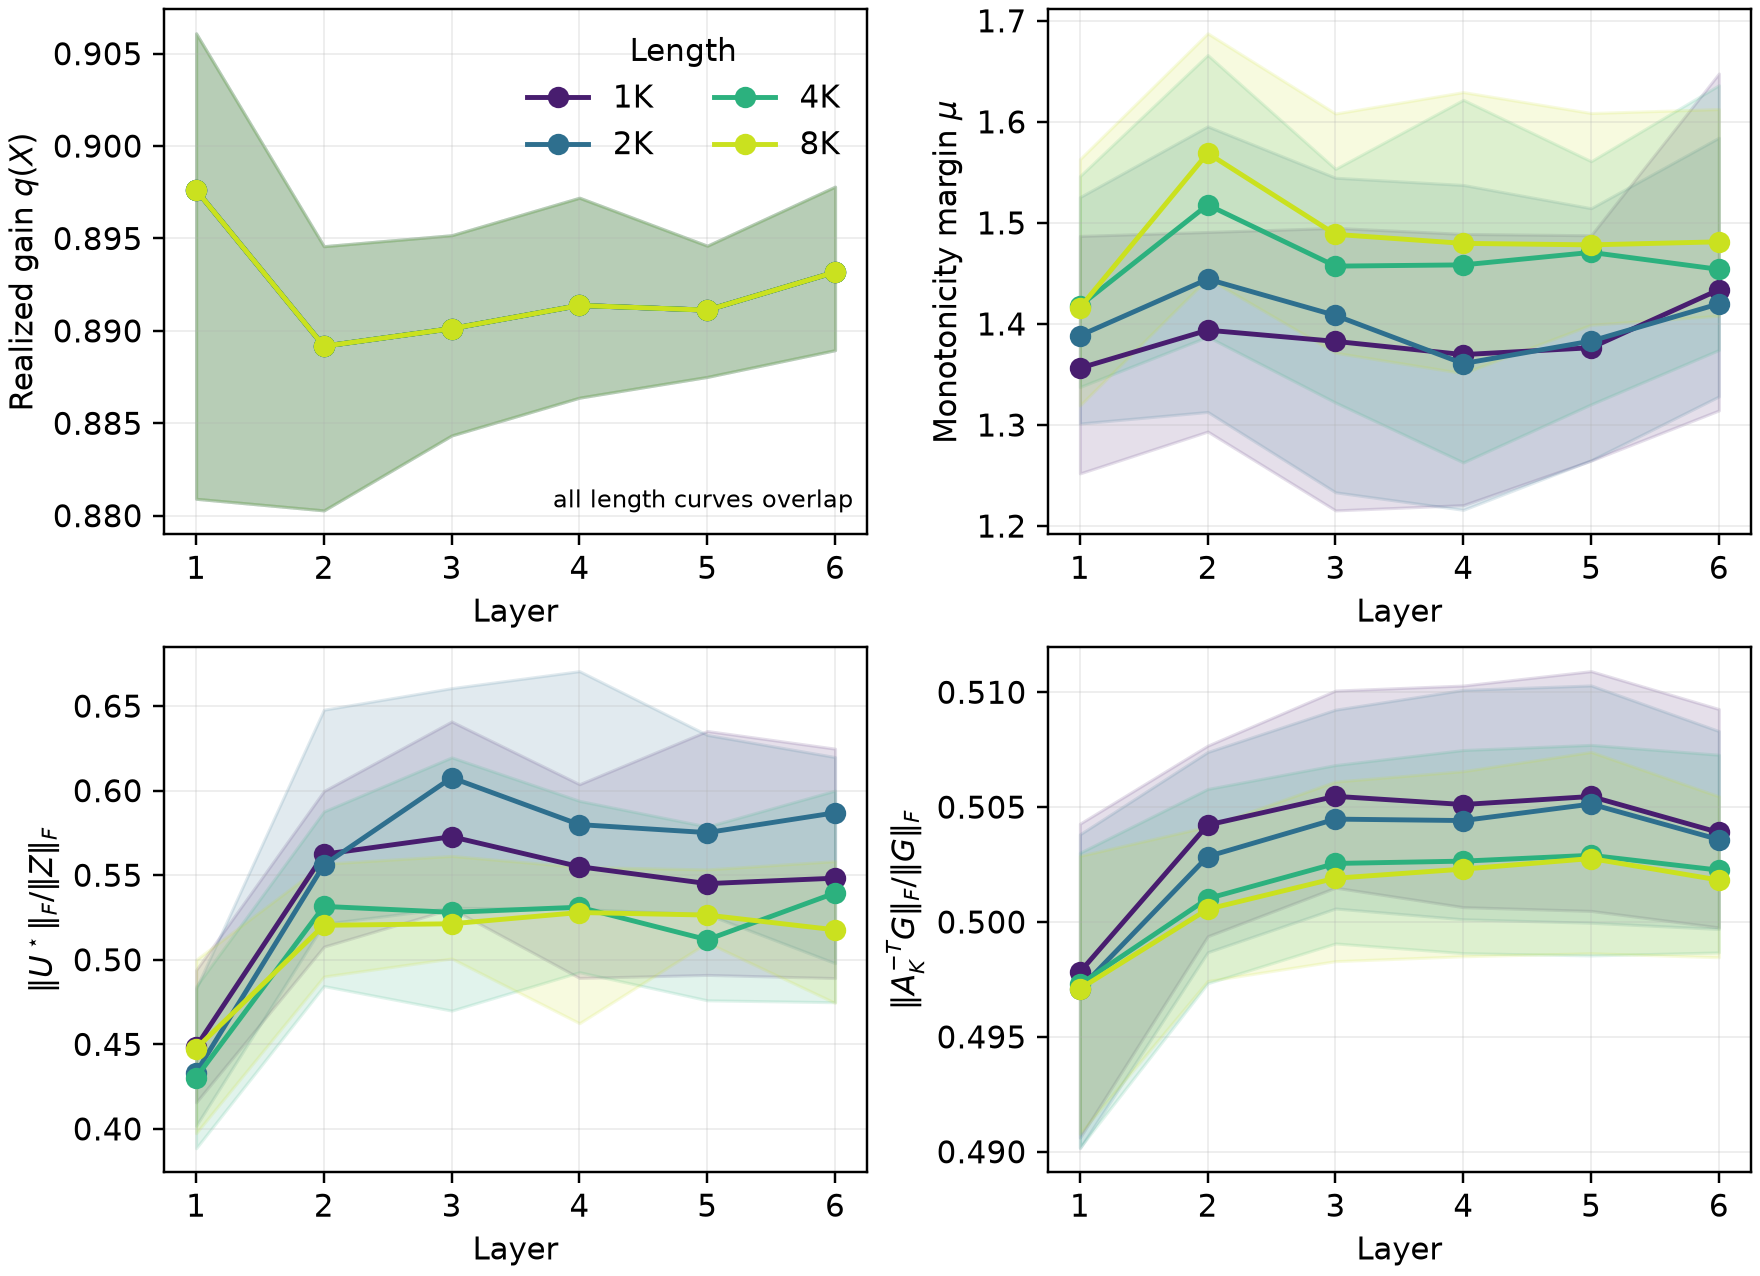
\includegraphics[width=0.58\linewidth]{certificate_length_depth.png}
\caption{Per-layer certificate diagnostics from three trained LRA Text
checkpoints.  Curves show medians and shaded 10th--90th percentiles over
held-out token-stream probes and heads.  All four realized-gain curves overlap;
the $8$K points are operator-level stress measurements.}
\label{fig:certificate-length-depth}
\end{figure}

\section{Mixer-Core MAC Accounting}
\label{app:mixer-macs}

Table~\ref{tab:mixer-macs} reports the leading sequence-dependent matrix
contractions per sample, accumulated over all mixer layers.  For depth $L$,
$H$ heads, head width $d=D/H$, and rank $r=32$, the accounting is
\begin{equation}
    \operatorname{MAC}_{\mathrm{LSSO}}=2LHN r(r+d),
    \qquad
    \operatorname{MAC}_{\mathrm{MHA}}=2LHN^2d.
\label{eq:mixer-mac-accounting}
\end{equation}
The LSSO count comprises two token--rank frame passes and two frame--content
contractions; the MHA count comprises $QK^\T$ and the attention--value product.
Feature projections, elementwise maps, MLPs, task heads, and the
$N$-independent compact factorizations and solves are excluded from both
columns.

\begin{table}[H]
\centering
\footnotesize
\setlength{\tabcolsep}{4.5pt}
\caption{Sequence-dependent mixer-core GMACs per sample at each task's maximum
length, accumulated over all encoder layers.  The final column reports LSSO as
a percentage of MHA.}
\label{tab:mixer-macs}
\begin{tabular}{lrcrrr}
\toprule
Task & $N$ & $D/L/H$ & LSSO & MHA & LSSO/MHA (\%) \\
\midrule
\multicolumn{6}{l}{\emph{GenomicBenchmarks}} \\
Coding vs. intergenomic & 200  & $128/4/4$ & $0.0131$ & $0.0410$ & $32.0$ \\
Human or worm           & 200  & $128/4/4$ & $0.0131$ & $0.0410$ & $32.0$ \\
Mouse enhancers Ensembl & 4776 & $128/4/4$ & $0.3130$ & $23.3576$ & $1.3$ \\
Human enhancers Cohn    & 500  & $128/4/4$ & $0.0328$ & $0.2560$ & $12.8$ \\
Human enhancers Ensembl & 573  & $128/4/4$ & $0.0376$ & $0.3362$ & $11.2$ \\
Human regulatory        & 802  & $128/4/4$ & $0.0526$ & $0.6586$ & $8.0$ \\
Human non-TATA promoters & 251 & $128/4/4$ & $0.0164$ & $0.0645$ & $25.5$ \\
Human OCR Ensembl       & 593  & $128/4/4$ & $0.0389$ & $0.3601$ & $10.8$ \\
\midrule
\multicolumn{6}{l}{\emph{Long Range Arena}} \\
ListOps                 & 2048 & $128/6/8$ & $0.3020$ & $6.4425$  & $4.7$ \\
Text                    & 4096 & $256/6/8$ & $0.8053$ & $51.5396$ & $1.6$ \\
Retrieval               & 4000 & $128/6/8$ & $0.5898$ & $24.5760$ & $2.4$ \\
Pathfinder-32           & 1024 & $256/6/4$ & $0.1510$ & $3.2212$  & $4.7$ \\
\bottomrule
\end{tabular}
\end{table}

\section{CUDA Implementation Details}
\label{app:cuda}

\subsection{Execution contract}

The native backend implements \textsc{Dynamic} with Rank-Rotary for inference
and first-order training and is algebraically equivalent to
Section~\ref{sec:method}.  It accepts FP16 or FP32 activations with FP32 learned
parameters.  The \textsc{Static}, \textsc{Zero}, and Rank-Rotary-off ablations
remain reference-only.

The joint input projection in Equation~\eqref{eq:input-projection} produces
contiguous FP32 relation and content coordinates with TF32 enabled on
supporting hardware.  The separate output projection uses FP16 Tensor-Core
operands with FP32 accumulation before casting back to the activation dtype.

The schedule supports
\begin{equation}
    r\in\{16,32,48,64\}
\end{equation}
and any positive head width $d$ within allocation and launch limits, including
$r>d$.  Runtime right-hand-side panels have width 32 with zero-filled tails.

Boolean validity masks have shape $[B,N]$, and position identifiers have shape
$[N]$ or $[B,N]$.  Invalid projected rows are zeroed before every compact
statistic, all sample-dependent normalizations use
$\sqrt{n_{\mathrm{valid}}}$, and invalid output rows are zeroed again.  This
covers gapped padding and entirely masked samples in one generic schedule.
Position identifiers and valid-token counts are metadata rather than
differentiable inputs.

\subsection{Lowering to tiled kernels}

The forward pass begins with a rank-phase schedule that constructs the
Rank-Rotary sine and cosine table.  Consecutive default positions are cached by
device, rank, and sequence length; explicit positions use an invocation-local
table.  One relation-input kernel combines phase rotation,
$1/\sqrt{n_{\mathrm{valid}}}$ normalization, detached common scaling, and
storage of the scaled relation coordinates.

The soft frame uses the Gram--Cholesky form algebraically equivalent to the
positive-diagonal reduced QR in Equation~\eqref{eq:soft-frame}.  Short
sequences use a single-block FP32 Gram reduction.  At 32 or more 32-token
tiles, independent partial Grams are reduced in ascending token order before
the same Cholesky factorization.  Tiled triangular solves then materialize the
frame.  The cross-moment $Z=P^\T C$ is produced in independent token and
right-hand-side tiles using FP16 Tensor-Core multiplicands and FP32
accumulation; no more than 64 token partials are live at once.

A compact-core kernel evaluates
\begin{equation}
    \Theta=\Theta_0+\frac{ZW_{\mathrm{drive}}}
                            {\sqrt{n_{\mathrm{valid}}}},
\end{equation}
constructs $L$ and $\Omega$, forms $LL^\T$ using IEEE FP32 FMA, assembles
$\I+K$, and performs partial-pivot LU factorization.  Separate 32-column FP32
solve panels compute $U^\star=(\I+K)^{-1}Z$.  The final tiled kernel directly
evaluates
\begin{equation}
    Y=\eta C+P[2U^\star-(1+\eta)Z].
\end{equation}
Thus neither the Cayley matrix $M$ nor a token-space transition matrix is
stored.

\subsection{Analytic backward and activation storage}

Training records a private contiguous FP32 tape per sample and head together
with one-based INT32 LU pivots.  The backward reuses the saved LU factors to
apply the transposed equilibrium solve, then evaluates analytic VJPs for the
dynamic core, accretive parameterization, compact cross-moment, soft frame, and
Rank-Rotary transform.  It does not differentiate through an unrolled solver.
The token-level frame and relation derivatives are fused, so the
single-consumer frame adjoint remains on chip rather than making a global
$[BH,N,r]$ round trip.  The complement reduction reconstructs its
frame--content term in FP32 within an existing compact kernel.  Buffers are
reused after their last consumer: the compact-core matrix adjoint becomes the
frame adjoint, and compact-state partial storage is overwritten after its
reduction.

Let $S=BH$, $T_{32}=\lceil N/32\rceil$,
$T_{64}=\lceil N/64\rceil$, $Q=\lceil d/32\rceil$, and
$C_T=\min(T_{32},64)$.  Excluding packed input, output, returned gradients,
Rank-Rotary phase tables, and allocator bookkeeping, the saved training tape
contains
\begin{equation}
    W_{\mathrm{train}}
    =S(2Nr+3r^2+2rd+1)
\label{eq:cuda-training-tape}
\end{equation}
FP32 values and $Sr$ INT32 pivots.  The compact inference workspace contains
\begin{equation}
    W_{\mathrm{infer}}
    =S(Nr+2r^2+2rd+1)
\label{eq:cuda-inference-workspace}
\end{equation}
FP32 values, plus $Sr$ transient INT32 pivots.
Rank-Rotary phase storage is additional: a shared table contains $Nr$ FP32
values, while per-sample positions require $BNr$.  Default consecutive-position
tables live in a bounded persistent cache; explicit position tables are
invocation-local.

The long-sequence Gram schedule has the logical live storage
\begin{equation}
    W_{\mathrm{Gram}}
    =S T_{32}\frac{r(r+1)}{2}
\label{eq:cuda-gram-workspace}
\end{equation}
in FP32.  Tape-producing calls with $r\in\{16,32,48\}$ place these partials in
the not-yet-materialized frame region; inference and $r=64$ training allocate
them separately.  The cross-moment producer uses
\begin{equation}
    W_{\mathrm{cross}}=S Q C_T r\,32
\label{eq:cuda-cross-workspace}
\end{equation}
FP32 values, and its lifetime does not overlap the Gram temporary.  Native
backward scratch contains
\begin{equation}
    W_{\mathrm{backward}}
    =S(T_{64}rd+T_{64}+3rd+2r^2)
\label{eq:cuda-backward-workspace}
\end{equation}
FP32 values.  These formulas describe the principal tape/workspace and the
explicitly listed scratch tensors owned by the native mixer; full-module peak
memory additionally includes phase storage, feature projections, external
autograd state, returned gradients, and allocator caching.

\subsection{Numerical and build coverage}

The contract-6 backend used for the reported experiments follows a fixed mixed TF32/FP16-Tensor-Core/FP32 contract. The current source uses contract 8 (BF16 ordinary multiplicands, FP16 phase storage, and FP32 sensitive arithmetic); the reported experiments have not been rerun under that contract.  The
joint input projection uses TF32 where supported.  Selected compact
contractions and the readout use FP16 multiplicands with FP32 accumulation.
Rank-Rotary phases, the soft-frame Gram and Cholesky factorization, the
one-ULP-interiorized complement, $LL^\T$, LU factorization, and triangular
solves remain FP32.  This fixed precision partition applies to every supported
configuration.

FP64 evaluation of the sole reference operator is the numerical oracle.  The
CUDA acceptance envelope requires finite outputs and gradients, forward
relative $\ell_2$ error at most $5\times10^{-3}$, and input- and
parameter-gradient relative $\ell_2$ error at most $10^{-2}$.  The oracle suite
covers all four ranks,
non-tile-aligned head widths, lengths through 4776, the
$N=4096,D=256,H=8,r=32$ long-sequence setting, parallel Gram reduction,
batch-specific positions, gapped masks, entirely masked samples, and agreement
between inference and tape-producing forward entry points.  Acceptance is
defined by these mixed-precision error envelopes.

CUDA 12.8 with cuBLASDx and cuSolverDx from MathDx 25.12.1 builds separate
artifacts for
\begin{equation}
    \mathrm{SM}\in\{75,80,86,87,89,90,100,120\}.
\end{equation}
Each binary records its compiled SM and numerical contract.  Physical latency
and numerical measurements use the RTX 5070 Ti specified below.

\subsection{Wall-clock protocol}

Table~\ref{tab:cuda-wall-clock} was measured under WSL2 on one NVIDIA GeForce
RTX 5070 Ti (16 GB, SM120), driver 610.88, PyTorch 2.11.0+cu128, CUDA 12.8, and
native contract version 6.  Training measurements use training mode, while
inference measurements use evaluation mode.  Each process pregenerates a
contiguous input tensor and enables TF32.  LSSO uses the default \textsc{Dynamic} core
with Rank-Rotary, consecutive positions, and no padding mask.
The comparison is PyTorch \texttt{nn.MultiheadAttention} with bias, zero
dropout, batch-first layout, and \texttt{need\_weights=False}, using PyTorch's
Flash SDPA forward and backward kernels.

The timed boundary includes both operators' input and output projections, but
excludes residual connections, MLPs, data loading, and optimizer updates.  The
forward--backward measurement differentiates a squared-mean scalar loss and
includes setting the input gradient to \texttt{None} every iteration and model
parameter gradients to \texttt{None} after each iteration.  No CUDA Graph or
\texttt{torch.compile} path is enabled.  Every configuration runs 50 untimed
warmup iterations, followed by seven repetitions of 100 iterations.  Each
repetition is bracketed by \texttt{torch.cuda.synchronize()}, and the reported
number is the median synchronized host wall-clock time per iteration.  Batch,
width, head count, rank, precision, and statistical protocol are fixed across
all sequence lengths and implementations.  The benchmark entry point is
\texttt{benchmarks/benchmark\_ball.py}.

{\small
\section{Figure Sources and Production}
The conceptual diagrams are supplied as vector PDFs.  Their matrix textures
and geometric illustrations are schematic and encode no experimental results.
Layout and export review used the Scientific Visualization skill from
Scientific Agent Skills \cite{kassis2026skills}; the drawing code and operator
content were written for this manuscript.  The tensor-flow diagrams in
ViT$^3$ \cite{han2026vit3} and the semantic color grouping in LION
\cite{afzal2025lion} informed the visual organization; no source artwork was
reused.  The existing certificate plot
reports the diagnostic protocol in Appendix~\ref{app:certificate-protocol}.

\begingroup
\small
\bibliographystyle{plain}
\bibliography{references}
\endgroup
}

\end{document}
